%*******10********20********30********40********50********60********70********80

\chap{Simulation of Residual Mechanical Capabilities Of ASR and DEF Expanded Concrete}

\section{General}

In this chapter, three-dimensional expanded concrete models are tested under uni-axial compression condition. The purpose of this study is for the prediction of the behavior and residual capacity of ASR or DEF expanded concrete, especially in uni-axial compression.

Displacement of loading boundary is controlled in this analysis. In each step of loading, the top boundary of the concrete model moves downwards 0.02mm.

\begin{figure}[ht]
\centering
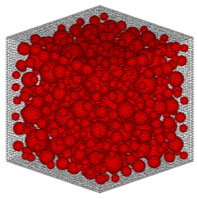
\includegraphics[width=.3\linewidth]{Files/Aggregate/A30.png}
  \caption{30\% Coarse Aggregate}
  \label{fig:A30_model}
\end{figure}

Figure \ref{fig:ASR_Loading} and Figure \ref{fig:DEF_Loading} here presented the internal stress condition of 2 example cases for ASR and DEF loading of Fixed boundary condition, seperately. In Figure , 100x100x100mm model with 30\% coarse aggregate is used, of which 75\% of all coarse aggregates are ASR reactived. While for DEF, same 100x100x100mm model with 30\% coarse aggregate is used, of which the center 75x75x75mm part has been given intensified DEF expansion, and gradually decrease until reaching the surface of the model.

It can be seen that with the increasing of vertical displacement applied to the expansion damaged models, compressive force generated in the concrete model,  and X shape cracking developed gradually until the failure of the structure is reached.

The internal stress reaction of ASR and DEF expanded concrete model is relatively close, but the maximum Compressive Strength and Elastic Modulus does show some of the differences.

And when considering free boundary condition loading, as presented in Figure \ref{}, the top and bottom of the concrete model can move freely in horizontal directions, thus the X-shape cracking pattern shown in fix boundary loading cases does now show up here.

%TODO: FREE Loading

Figure Free Loading Internal Stress

%A30P75FIX_3

\begin{figure}[ht]
\centering

    %*******
    \begin{subfigure}{.33\textwidth}
      \centering
      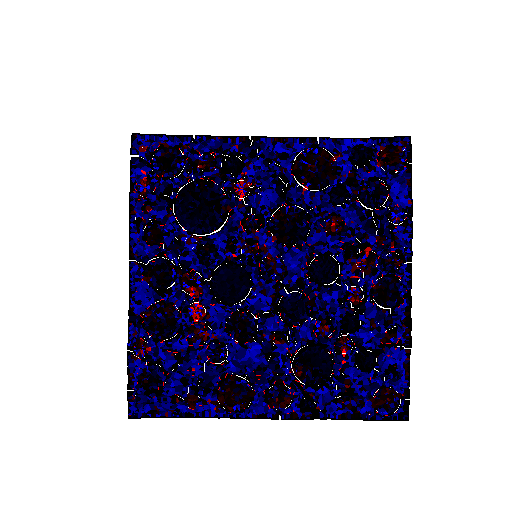
\includegraphics[width=1.0\linewidth]{Files/A30P75_3_IS/DEP50-STEP(020).png}
      \caption{Before Loading}
    \end{subfigure}%
    \begin{subfigure}{.33\textwidth}
      \centering
      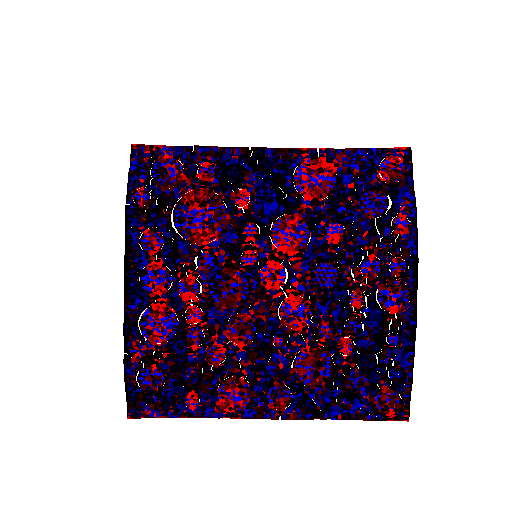
\includegraphics[width=1.0\linewidth]{Files/A30P75_3_IS/DEP50-STEP(040).png}
      \caption{Loading Step 20}
      \end{subfigure}%
      %*******
      \begin{subfigure}{.33\textwidth}
        \centering
        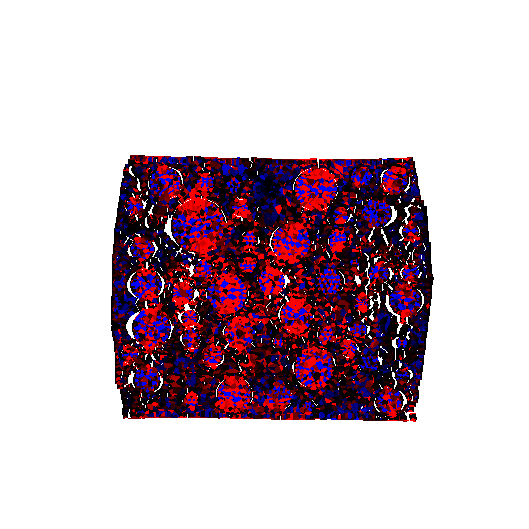
\includegraphics[width=1.0\linewidth]{Files/A30P75_3_IS/DEP50-STEP(060).png}
        \caption{Loading Step 40}
      \end{subfigure}
      %*******

    %*******
    \begin{subfigure}{.33\textwidth}
      \centering
      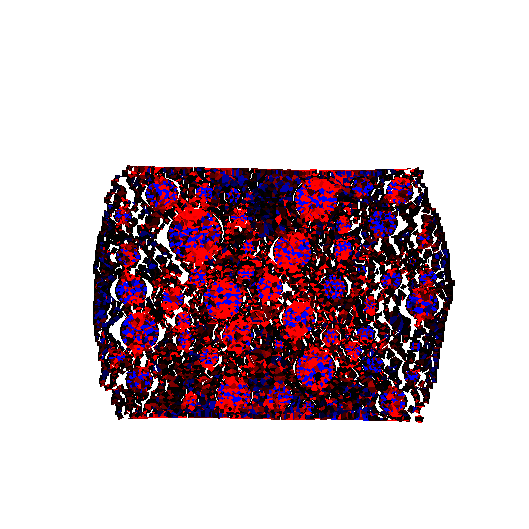
\includegraphics[width=1.0\linewidth]{Files/A30P75_3_IS/DEP50-STEP(080).png}
      \caption{Loading Step 60}
    \end{subfigure}%
    \begin{subfigure}{.33\textwidth}
      \centering
      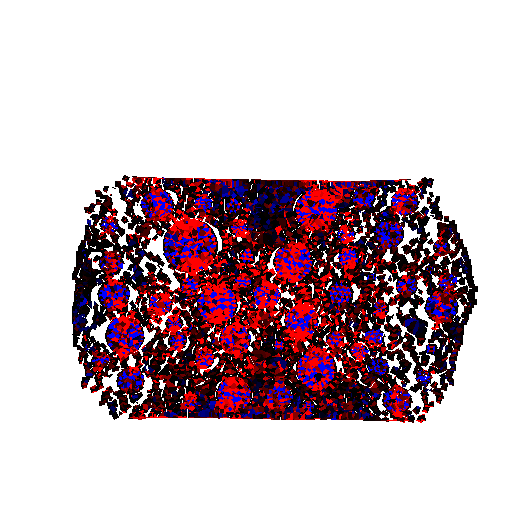
\includegraphics[width=1.0\linewidth]{Files/A30P75_3_IS/DEP50-STEP(100).png}
      \caption{Loading Step 100}
      \end{subfigure}%
      %*******
      \begin{subfigure}{.33\textwidth}
        \centering
        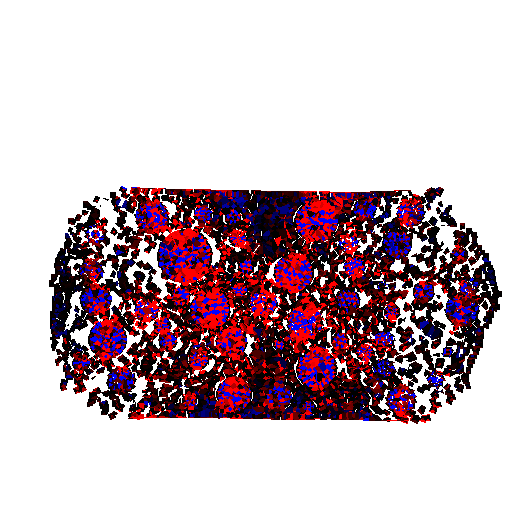
\includegraphics[width=1.0\linewidth]{Files/A30P75_3_IS/DEP50-STEP(120).png}
        \caption{Loading Step 120}
      \end{subfigure}
      %*******

  \caption{ASR Loading}
  \label{fig:ASR_Loading}
\end{figure}

\begin{figure}[ht]
\centering

    %*******
    \begin{subfigure}{.33\textwidth}
      \centering
      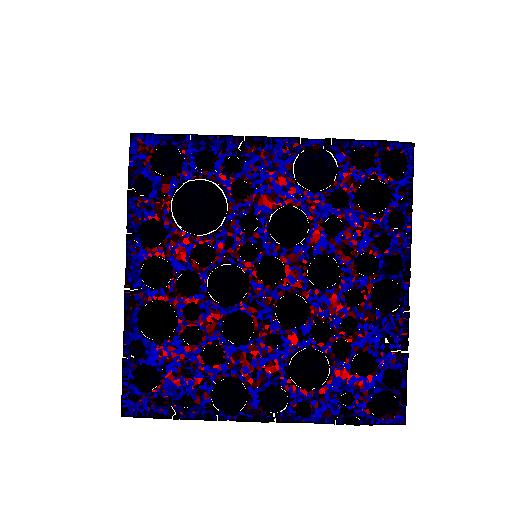
\includegraphics[width=1.0\linewidth]{Files/A30X-5C_3_IS/DEP50-STEP(020).png}
      \caption{Before Loading}
    \end{subfigure}%
    %*******
    \begin{subfigure}{.33\textwidth}
      \centering
      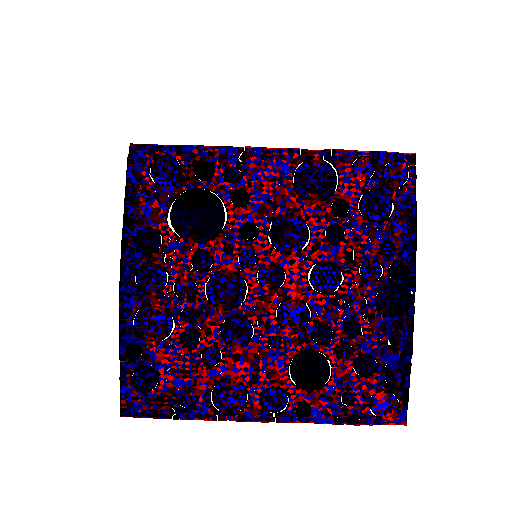
\includegraphics[width=1.0\linewidth]{Files/A30X-5C_3_IS/DEP50-STEP(040).png}
      \caption{Loading Step 20}
      \end{subfigure}%
      %*******
      \begin{subfigure}{.33\textwidth}
        \centering
        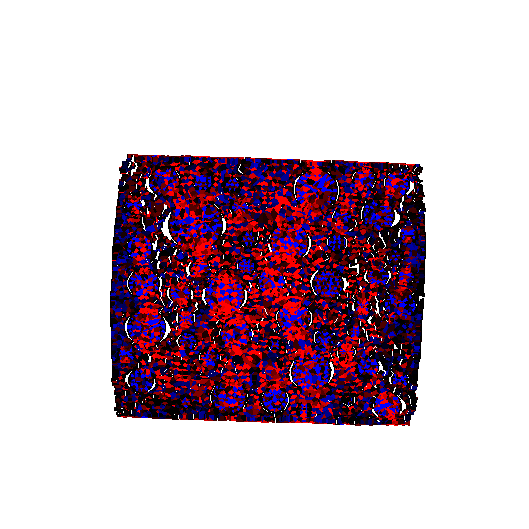
\includegraphics[width=1.0\linewidth]{Files/A30X-5C_3_IS/DEP50-STEP(060).png}
        \caption{Loading Step 40}
      \end{subfigure}
      %*******

    %*******
    \begin{subfigure}{.33\textwidth}
      \centering
      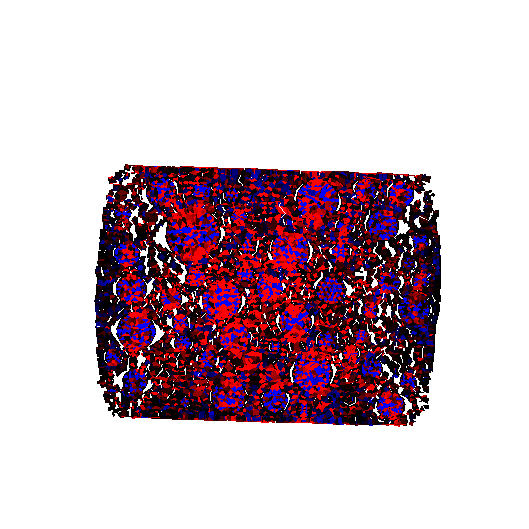
\includegraphics[width=1.0\linewidth]{Files/A30X-5C_3_IS/DEP50-STEP(080).png}
      \caption{Loading Step 60}
    \end{subfigure}%
    \begin{subfigure}{.33\textwidth}
      \centering
      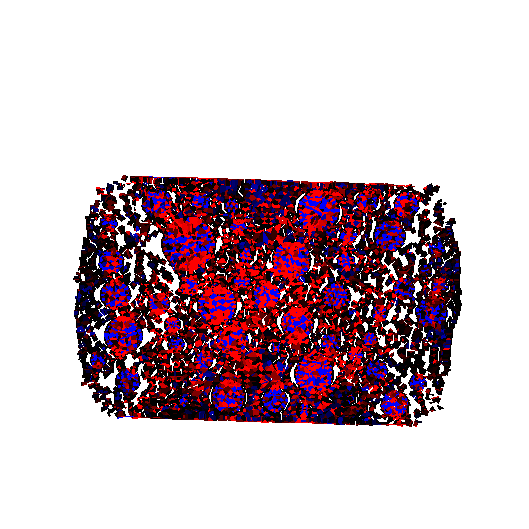
\includegraphics[width=1.0\linewidth]{Files/A30X-5C_3_IS/DEP50-STEP(100).png}
      \caption{Loading Step 100}
      \end{subfigure}%
      %*******
      \begin{subfigure}{.33\textwidth}
        \centering
        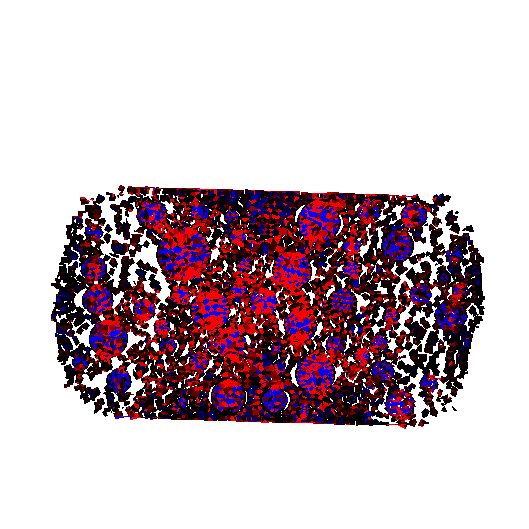
\includegraphics[width=1.0\linewidth]{Files/A30X-5C_3_IS/DEP50-STEP(120).png}
        \caption{Loading Step 120}
      \end{subfigure}
      %*******

  \caption{DEF Loading}
  \label{fig:DEF_Loading}
\end{figure}


As for the displacement change in each step, Compressive Strength is also recorded to show the residual mechanical properties of the expanded model. Besides, Elastic Modulus will also be calculated from the plotting of the load-displacement graph.


\subsection{Overview of Experimental Results of Residual Mechanical Properties After ASR Expansion}

\subsection{Overview of Experimental Results of Residual Mechanical Properties After DEF Expansion}
